\documentclass[11pt]{article}
\usepackage[utf8]{inputenc}
\usepackage{cs170}
\usepackage{derivative}
\usepackage{mathdots}

\def\title{}
\def\duedate{INSERT DUE DATE}


\begin{document}
\question{Median Filtering}

Recall that a convolutional kernel in image contexts involves calculating the sum of the elementwise products of the kernel with a window of pixels in the image, then sliding the kernel across the image, repeating the process for every pixel in the image.

\begin{subparts}
    \subpart Consider the following 3x3 kernel:
    $$\frac{1}{9} \begin{bmatrix}
    1 & 1 & 1 \\
    1 & 1 & 1 \\
    1 & 1 & 1
    \end{bmatrix}$$

    This is often referred to as a "box-blur" kernel. Why does it have a blurring effect?


    \subpart Now consider a related technique, known as \emph{median filtering}. Here, for a given window of pixels, the center pixel is replaced with the median of the pixels in the window. This process is then repeated across the entire image, just as is done with convolution.
    
    For your curiosity, depicted below are the results of applying 3x3 filters to an image (original left, box-blur center, median right):
    \begin{figure}[h] \centering
        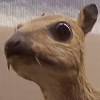
\includegraphics[width=0.3\textwidth]{orig.png}
        
\includegraphics[width=0.3\textwidth]{box_blur.png}
        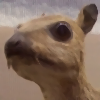
\includegraphics[width=0.3\textwidth]{median_filtered.png}
    \end{figure}

    Can you think of a scenario where median filtering would be preferable to box-blur filtering? What about the other way around?


    \subpart For ConvNets, are median filters similar to convolutional layers? Are they still useful? Why or why not?


    \subpart Consider the infinite zero matrix 
    $$\mathbf{0} = \begin{bmatrix}
        \ddots & \vdots & \vdots & \iddots \\
        \cdots & 0 & 0 & \cdots \\
        \cdots & 0 & 0 & \cdots \\
        \iddots & \vdots & \vdots & \ddots
    \end{bmatrix},$$ which, for this problem, represents a bitmap of constant color. Now suppose each pixel in the image is independently at random flipped to $1$ with probability $p < 0.2$, representing random noise. What is the expected result of applying a $3 \times 3$ box-blur filter to this newly noised image? What about a $3 \times 3$ median filter? Assume the stride length is at least 3 (so there is no overlap).
    
    Do your answers to (b) and (c) now change?

    \subpart Let $K \times K$ denote filter size, $P$ padding size, $S$ stride length, and suppose we are operating on an image of size $H \times W$. What is the runtime complexity of convolution? How about median filtering? Assume no results are cached across different pixels.

    \emph{Hint: You can find the median of $n$ numbers in $O(n)$ time.}


\end{subparts}

\newpage

\question{Weighted Cross-Entropy}
	Recall that cross-entropy loss is given by
    $$
    \mathcal{L}(y, \hat{y}) = - y \log \hat{y} - (1 - y) \log (1 - \hat{y}),
    $$
    where $y$ is the ground truth label and $\hat{y}$ is the predicted probability that the label is $1$.

    \begin{subparts}
        \subpart Suppose $p$ is the ground-truth probability of a positive sample. Find the value of $\hat{y}$ that minimizes the expected loss
        $$\mathbf{E}_{y \sim \text{Bernoulli}(p)}\left[\mathcal{L}(y, \hat{y})\right]$$ by taking the derivative with respect to $\hat{y}$ and setting it to zero.

        \newpage
        \subpart Now, consider how the model is affected by $p$. Below is the graph of $\mathbf{E}[\mathcal{L}]$ as a function of $\hat{y}$ for $p=0.5$, $p=0.05$, and $p=0.005$. From this, comment on what problems may arise when using binary cross-entropy loss (you do not need to show these rigorously).
        \begin{figure}[h] \centering
            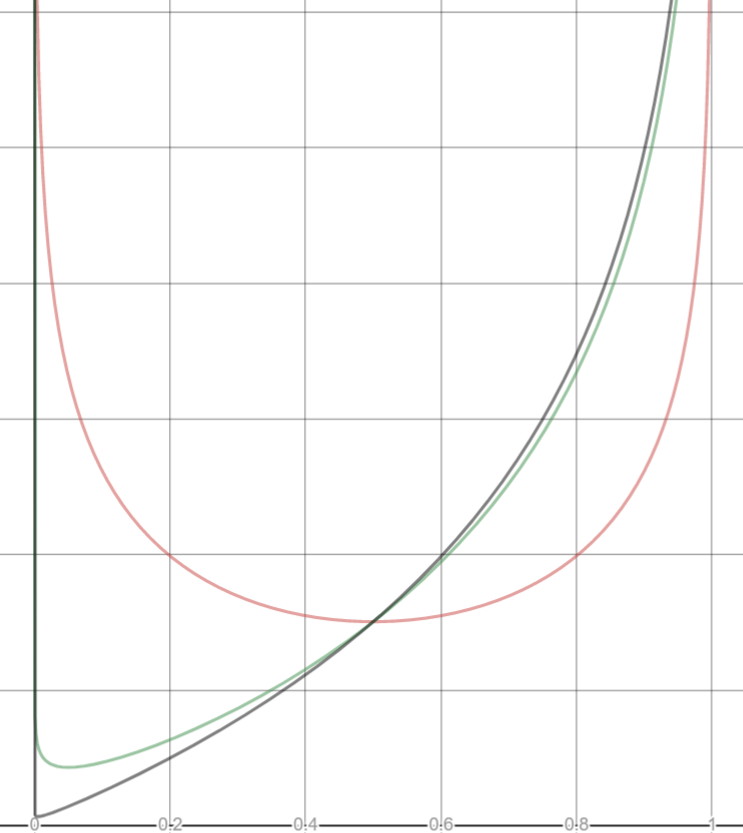
\includegraphics[width=0.5\textwidth]{binary-cross-entropy-pqr.png}
        \end{figure}


        \newpage
        % Find 
        % $$\pdv{}{p} \mathbf{E}_{y \sim \text{Bernoulli}(p)}[\mathcal{L}(y, \hat{y})]$$
        % using the optimal value of $\hat{y}$ found in the previous subpart. From this, what values of $p$ will be problematic for our model's predictions from a convergence perspective? (You do not need to show this rigorously.)

        % \answer{
        %     \begin{align*}
        %         \pdv{}{p} \mathbf{E}_{y \sim \text{Bernoulli}(p)}[\mathcal{L}(y, \hat{y})]
        %         &= \pdv{}{p} \left(- p \log \hat{y} - (1 - p) \log (1 - \hat{y})\right) \\
        %         &= - \log \hat{y} + \log(1 - \hat{y}) \\
        %         &= \log \frac{1 - \hat{y}}{\hat{y}} \\
        %         &= \log \frac{1 - p}{p}.
        %     \end{align*}
        %     When $\hat{y}$ is close to $0$ or $1$, the loss becomes very unstable. This is the case when $p$ is close to $0$ or $1$, indicating an unbalanced distribution. This means that we will need to have an extremely small learning rate to ensure convergence, which will slow training significantly.
        % }

        \subpart Suppose we want to modify the loss function to be more robust to unbalanced distributions. One way to do this is to introduce a hyperparameter $\alpha$, which we can use to penalize incorrect predictions more heavily for the minority class (or equivalently, less heavily for the majority class). This is called \emph{weighted cross-entropy} and is given by
        $$
        \mathcal{L}_\alpha(y, \hat{y}) := - \alpha y \log \hat{y} - (1 - y) \log (1 - \hat{y}).
        $$
        \begin{enumerate}
            \item[(i)] Find the value of $\hat{y}$ that minimizes the expectation of this loss. Remember that the ground-truth probability of a positive sample is $p$, and $y \sim \text{Bernoulli}(p)$.
            
            
            \item[(ii)] Use the value of $\hat{y}$ from part (i) to find $\alpha$ in terms of $p$ such that, when averaged over sufficiently many samples, both the minority and majority classes contribute to the total loss equally.
            
            \emph{Note: This derivation is quite difficult, but the final answer should be relatively simple. Feel free to use a symbolic or graphing calculator.}
            
        \end{enumerate}
    \end{subparts}

    \newpage
    \question{Basic Pitch}
        In 2022, Spotify released a free software known as Basic Pitch that can translate raw audio files to digitized sheet music (known as MIDI). You can find the paper at \url{https://arxiv.org/pdf/2106.02769.pdf}.
        \begin{subparts}
            \subpart The paper describes median filtering as a common technique for denoising audio, using a 1D median filter (audio files are essentially one-dimensional time series of frequencies). Suppose we only had access to square median filters. How can we use these square median filters to denoise audio samples?

            \emph{Hint: How do we generally visualize functions of a single variable? Can you apply that here?}

            \subpart Basic Pitch uses various sophisticated losses to determine the quality of the generated MIDI files, but they are all binary. For example, consider the question "Is the note at a given frequency being played?" How does this relate to what you learned in problem (2)?
            
        \end{subparts}

\end{document}
